\documentclass[12pt,a4paper]{article}
\usepackage[utf8]{inputenc}
\usepackage{amsmath}
\usepackage{amsfonts}
\usepackage{amssymb}
\usepackage{graphicx}
\usepackage[breaklinks,colorlinks,linkcolor=black,
            citecolor=black,urlcolor=black]{hyperref}
\author{Keshava Rangarajan}
\title{Deep Learning Elegantly Chapter 0 Deep Origins}
\begin{document}
\section{Deep Origins}
\paragraph{}
The story of deep learning, as viewed by the general public, is a recent phenomenon. In reality it is actually a long and old story rooted in humankind’s fascination with understanding reasoning: where it occurred, the processes­­associated with it, their interconnections, if and how it could be recreated.
\paragraph{}
\noindent
Though it is now common knowledge that
\begin{itemize}
\item Thinking occurs in the brain
\item Our brains have billions of interconnected neurons or brain cells 
\item These brain cells or neurons work collectively as a connected “intelligence” network to enable us to think, to feel, and, to act
\end{itemize}
this common knowledge is actually the result of millennia of “not so common” research and investigation; research that has been punctuated by short, intense bursts of progress and long, debilitating periods of regress.

\paragraph{}
Historical evidence shows that the brain has been a constant object of study from antiquity (B.C.E). Scientists from ancient times, across several civilizations, studied the brain to comprehend its functions and used that knowledge for medical purposes.
(reference: images of Indian historical figures who studied the brain including Charaka, Sushruta, trepanation in Harappa: https://bit.ly/38tt9L5; Babylonian, Egyptian efforts). 

\paragraph{}
In the early common era (C.E) times, scientists and researchers continued their efforts, and by the first century, a general physical description of the brain was available to the scientific community.  Basic structures such as the soft and hard layers encasing the brain were identified in addition to a basic classification/division of the brain into functional regions (subsequently called ventricles). 
\paragraph{}
Building upon this work, over the next few centuries, physicians concluded that mental activity occurred in the brain rather than the heart, thus concurring with what some pre common era scientists had already suggested.  What seems like a small step today was actually was a huge step forward for that time. They also concluded that the brain was the seat of the soul -- one of three "souls" found in the body, each associated with a principal organ.  Others were of the opinion that the brain was a cold, moist organ formed of sperm!

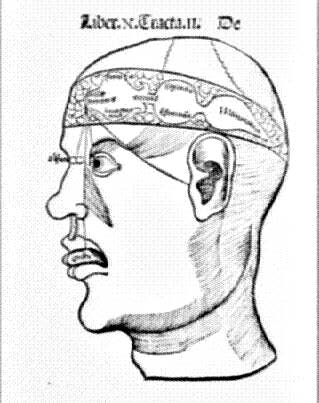
\includegraphics[scale=0.5]{307brain.jpg}\newline
image from \url{https://web.stanford.edu/class/history13/earlysciencelab/body/brainpages/307brain.jpg}\newline 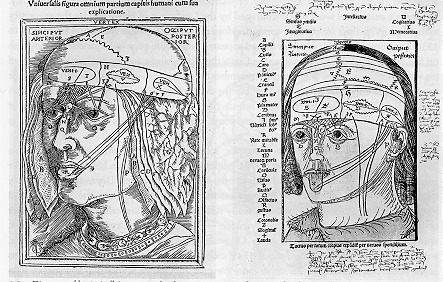
\includegraphics[scale=0.4]{brain85.jpg}\newline
image from \url{https://web.stanford.edu/class/history13/earlysciencelab/body/brainpages/85.gif}\newline

\paragraph{}
By the Middle Ages, the anatomy of the brain was broadly believed to be consolidated around three principle divisions.  Each division localized the site of different mental activity.  Imagination was believed to be located in the anterior ventricle, memory in the posterior ventricle, and reason located in between.  Yet, there was no consensus on where sensory processing, storing of the inputs, and the processing of the inputs received from the five senses (what was then called simply as “common sense”) resided.  Eleventh century scientists proposed that this “common sense” was housed in a "faculty of fantasy," that received "all the forms which are imprinted on the five senses."  Memory then preserved what common sense received.
\paragraph{}
But by the 14th century opinions changed. It was now believed that common sense lay in the middle of the brain.  Historical records also suggest that many fundamental questions regarding the functions of the brain (including those related to common sense) remained open to debate.  Indeed, this is true to this day, but at a far more nuanced level of detail. Such differences of opinion only underscore how little was known, then, of the brain's anatomy, let alone its physiology or functioning and now we continue to learn about it to this day.

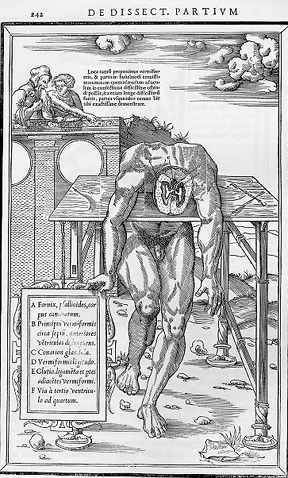
\includegraphics[scale=1]{brain185.jpg}\newline
image from \url{https://web.stanford.edu/class/history13/earlysciencelab/body/brainpages/brain185.jpg}
\newline
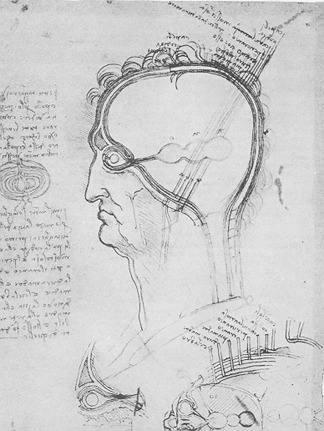
\includegraphics[scale=1]{davcranialnerves.jpg}\newline
image from \url{https://web.stanford.edu/class/history13/earlysciencelab/body/nervespages/davcranialnerves.gif}\newline
\paragraph{}
In the Renaissance period, physicians began to dissect the brain with much greater frequency, more so at the end of the fifteenth century. This, mid-sixteenth century anatomy illustration demonstrates such a dissection. Of particular note is the famous Leonardo da Vinci who also dissected and drew the brain.  Leonardo's images were considerably more anatomical in nature than a lot of his peers’. He systematically examined the relationship between the brain, the olfactory and the optical nerves through experiments with wax injections to help him to model the ventricles or sections of the brain.  
\paragraph{}
He sketched the brain from many different perspectives, looking closely at the ventricles and the origins of the nerves in the medulla.  Records suggest that the more he looked, the less he became sure about the function of each section! It is now known that one of his quests was to find the location of “common sense”.  The other was to locate the seat of the soul!\newline \newline
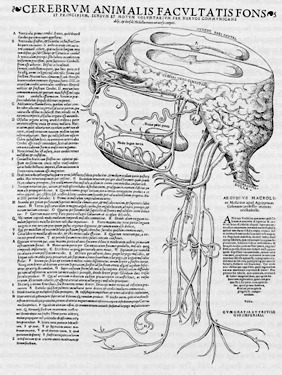
\includegraphics[scale=1]{renbrain151.jpg} \newline
image from \url{https://web.stanford.edu/class/history13/earlysciencelab/body/brainpages/renbrain151.gif}\newline
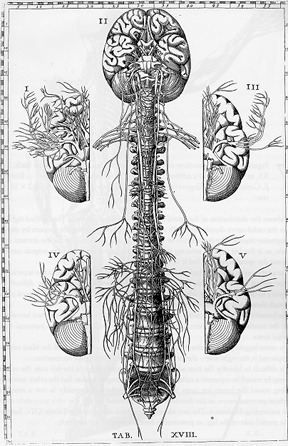
\includegraphics[scale=1]{brain195.jpg}\newline
image from \url{https://web.stanford.edu/class/history13/earlysciencelab/body/brainpages/195.gif}
\paragraph{}
Sixteenth and early seventeenth-century anatomists contributed a great deal to the physical description of the brain. Terms such as cerebrum, cerebellum and medulla were popularized. But they made few significant advances in their understanding of its functioning.  It was not until the 17th century that views on the anatomy of the brain changed significantly. Scientists began to advocate for more careful explorations of the cortex and the ventricles (two images of the brain, from the late sixteenth and mid-seventeenth centuries). The brain, finally, had a modern physiology, grounded in research and verifiable experiments. The basic concept and principles of neurology were established. The soul no longer had a home in the brain.
\paragraph{}
Then, in the late 19th century, Spanish physician Santiago Cajal (reference: figure of Santiago) formally identified neurons by staining and studying brain tissue in great detail. Cajal’s two brilliant insights — that every neuron in the brain is separate and that neurons communicate across synapses — came to be known as the neuron doctrine. Because that gap between neurons is too small to see through a light microscope, Camillo Golgi and other rigorous scientists of Cajal’s day at first dismissed the neuron doctrine as a fantasy. It would take another half-century until a new instrument, the electron microscope, could finally confirm what Cajal had seen in his mind’s eye — and carefully sketched out in thousands of stunning pen-and-ink diagrams.
\paragraph{}
He published his observations in 1894. Subsequently, in the early parts of the 20th century, researchers began the process of understanding exactly how these neuronal cells functioned. 
\newline
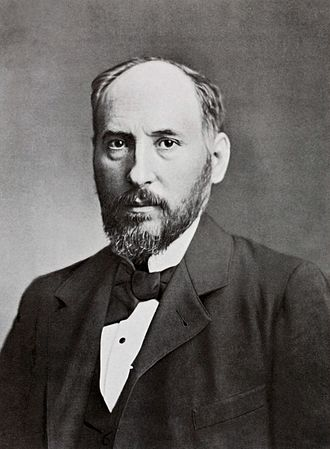
\includegraphics[scale=1]{Cajal-Restored.jpg}\newline
image from\newline
\url{https://en.wikipedia.org/wiki/Santiago_Ram%C3%B3n_y_Cajal#/media/File:Cajal-Restored.jpg}
\newline
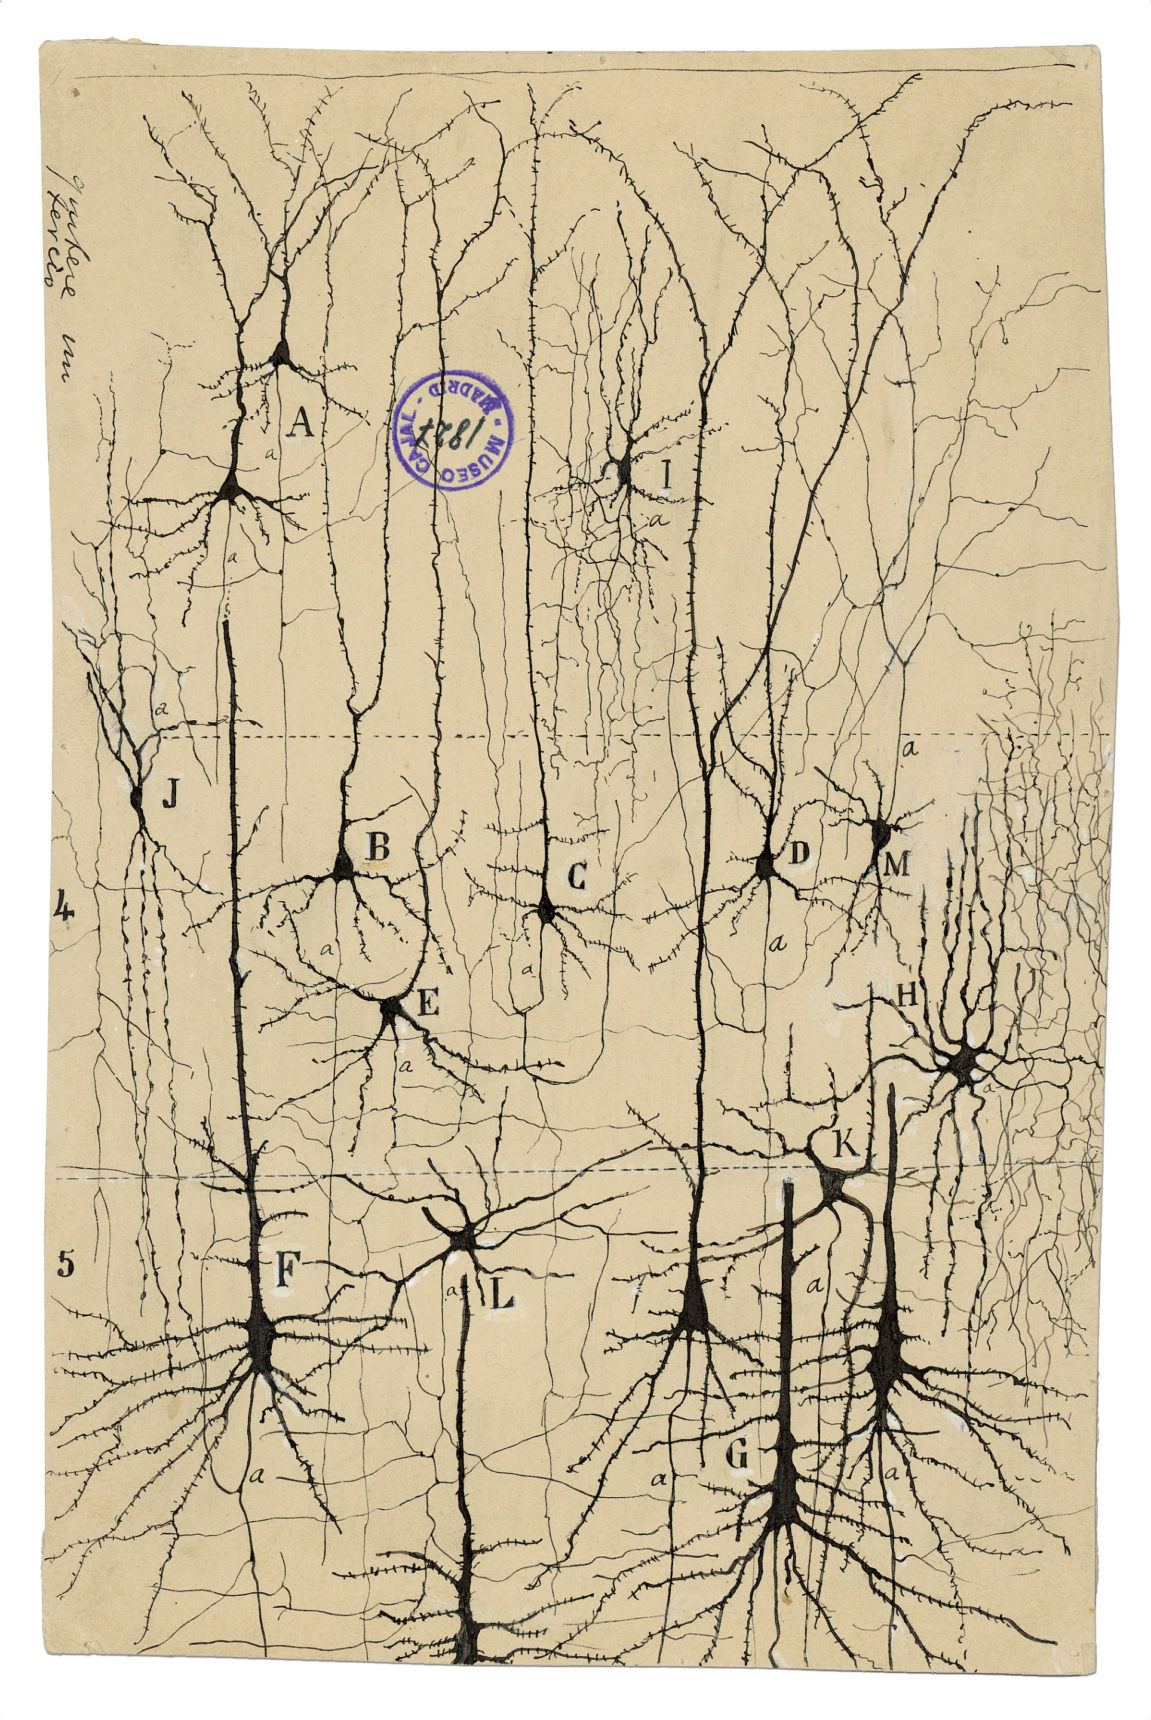
\includegraphics[scale=0.3]{cajal-neuron-drawing.jpg}\newline
image from \url{https://www.google.com/url?sa=i&url=https%3A%2F%2Fwww.quantamagazine.org%2Fwhy-the-first-drawings-of-neurons-were-defaced-20170928%2F&psig=AOvVaw3VoPk0ZuY-_kKKah11poCf&ust=1599863355072000&source=images&cd=vfe&ved=0CAIQjRxqFwoTCJiZw8vR3-sCFQAAAAAdAAAAABAg}
\paragraph{}
Cajal’s graceful drawings of neurons show them as separate, individual cells. He was the first to realize that the nervous system is not a network of continuous fibers, as was widely believed at the time.
\paragraph{}
Then a left shift event occurred! Computers arrived and gained momentum triggering ideas of transitioning research and experimentation from the physical world to the world of computers. Brain behavior research was considered an ideal candidate given the myriad constraints involved in acquiring specimen, performing physical experiments, deducing conclusions from results and verifying them.
\paragraph{}
Thus, in the mid 20th century, spurred by curiosity, inspired by the progresses made in the understanding of the brain and sensing the opportunity presented by their access to computing resources, Computer Scientists (a newly minted term) began experimenting with computerized simulations of the cognitive process of the brain. A subset of them chose to simulate cognitive processes by creating “artificial neurons” and then connecting them in “artificial neural networks” thus aiming to loosely mimic the physical organization and functioning of brain cells as seen in experiments involving small, localized sections of the brain.  
\paragraph{}
Warren McCulloch and Walter Pitts created a computer model using a combination of mathematics and algorithms to mimic the thought process. In their model small layers of artificial neurons passed input information to other neuronal layers until the final layer output values.  Then in his paper “The Perceptron: A Perceiving and Recognizing Automaton”, Rosenblatt shows the new avatar of McCulloch-Pitts neuron – ‘Perceptron’ that had true learning capabilities to do binary classification on its own. This inspired the revolution in research of shallow neural network for years to come. The Forward Propagation Artificial Neural Network had arrived!
\newline
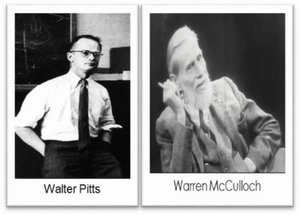
\includegraphics[scale=1]{walterpitts-and-warrenmcculloch.jpg}\newline
image from https://aiartists.org/ai-timeline-art\newline
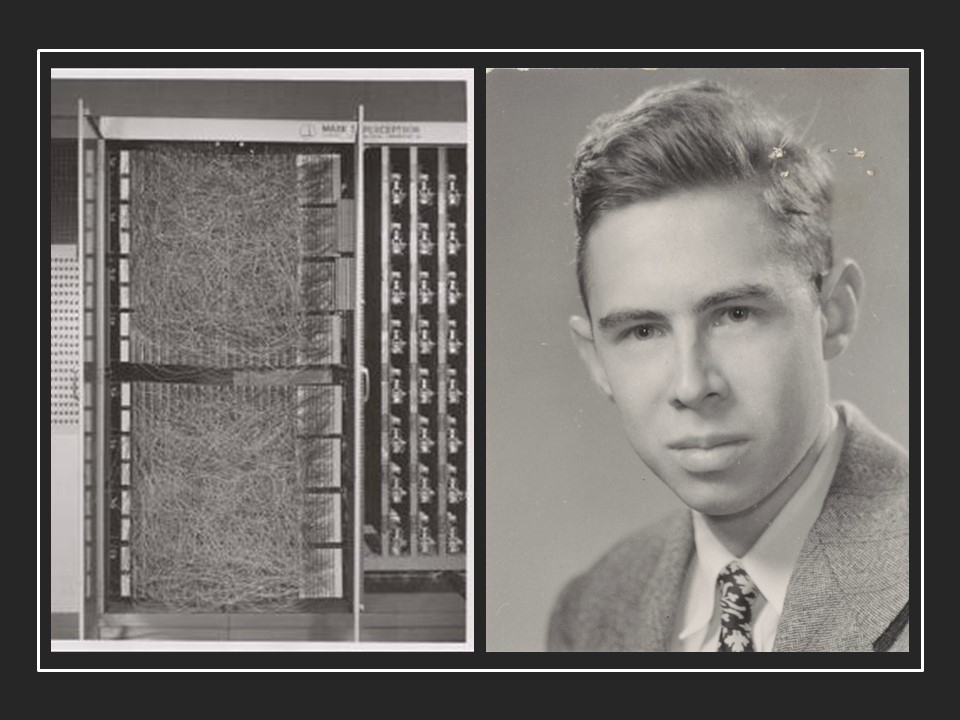
\includegraphics[scale=0.5]{franklin-rosenblatt.jpg}\newline
image from \url{https://machinelearningknowledge.ai/wp-content/uploads/2019/11/Frank-Rosenblatt-Perceptron.jpg}

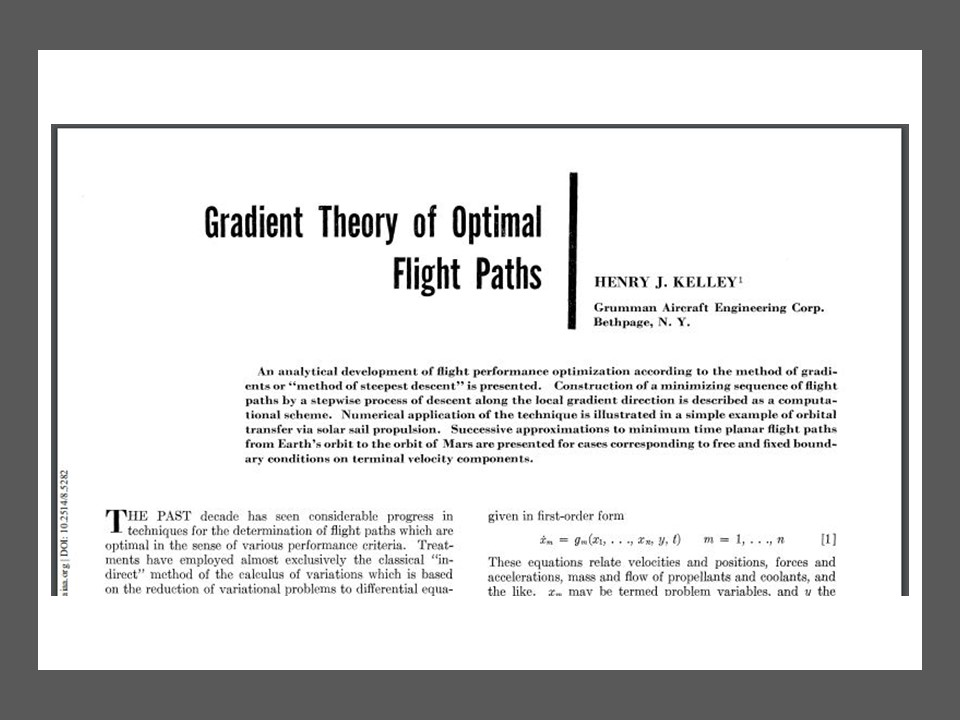
\includegraphics[scale=0.5]{henrykelley-backprop.jpg}\newline
image from \url{https://machinelearningknowledge.ai/wp-content/uploads/2019/11/Henry-J-Kelly-Backpropgation.jpg}

\paragraph{}
Following this, in 1960, Henry J. Kelley improved this model by developing the basics of Continuous Back Propagation. This approach introduced the notion of feedback control into the “learning” process. Although this key concept of back propagation existed in the early 1960s, it came of practical use only around 1985. 
You might have noticed by now that all of the work in Artificial Neural Networks  that we have discussed deal with what we would today call “shallow” networks i.e. Artificial Neural Networks that just had a few connected layers between the input and the output as well as being comprised of a relatively small number of connected neurons as a whole. But Deep Learning is defined as the process of processing signals and encoding knowledge using Deep Neural Networks which are large, deeply stacked, multi-layered networks of artificial neurons comprised of millions or more networked artificial neurons.  
\paragraph{}
So, when did this shift from simple shallow networks to complex deep networks occur? 
\paragraph{}
Well, the earliest efforts in developing deep learning algorithms actually date back to 1965, when Alexey Grigoryevich Ivakhnenko and Valentin Grigor'evich Lapa used models with polynomial (complicated equations!) activation functions, which were subsequently analyzed statistically. Then, just as things seemed to be gaining momentum, in 1970, Marvin Minsky and Seymour Papert published the book “Perceptrons” in which they show that Rosenblatt’s perceptron could not solve complicated functions like XOR. For such function perceptrons should be placed in multiple hidden layers which compromises the perceptron learning algorithm. This was a setback for “bottom up” AI. 
\paragraph{}
Around the same time, there was mounting sentiment that millions had been spent on AI research with the hope that it would provide a strategic technological advantage in the cold war, but little had come out of it. There was strong criticism from the US Congress. To add to this, in 1973, leading mathematician Professor Sir James Lighthill gave a damning health report on the state of AI in the UK!
\paragraph{}
Lighthill’s view was that machines would only ever be capable of an "experienced amateur" level of chess. Common sense reasoning and supposedly simple tasks like face recognition would always be beyond their capability. Funding for the industry was slashed, ushering in what became known subsequently as the AI winter. It was a period of intense setback in the research and development of Artificial Neural Networks and Artificial Intelligence (AI) in general. Severe cutbacks in funding plagued deep learning and AI research as a whole. 
\paragraph{}
However, despite the lean times, passionate researchers carried on the work without funding! Kunihiko Fukushima developed an artificial neural network, called Neocognitron in 1979, which used a multi-layered and hierarchical design. This design enabled computers to learn to recognize visual patterns. The backpropagation method was enhanced to feed errors in the output to influence and control the training of the models. This approach became widely popular when Seppo Linnainmaa wrote his master’s thesis, including FORTRAN code illustrating the backpropagation technique. The backpropagation concept was applied to neural networks and shown to work but made little impact. AI work then was primarily focused on top-down, rule based expert systems. Bottom up AI was still languishing. 
\paragraph{}
The first signs of revival were displayed when in 1985 Hinton and Williams demonstrated back propagation in a neural network which could provide interesting distribution representations. Yann LeCun followed this up by providing the first practical demonstration of backpropagation at Bell Labs in 1989 by combining convolutional neural networks with back propagation to read handwritten digits. The combination of convolutional neural networks with a backpropagation system was then used to read the numbers of handwritten checks spurring business interest. 
\paragraph{}
Interestingly, though this was a period of renewed interest, the 1985-90s actually are considered by the scientific AI community as the second lull in artificial intelligence. Hardware and software issues plagued the progress of research in neural networks and deep learning. Deep Learning algorithms while producing good results in lab conditions, struggled to scale well to industrial proportions, were quite unstable and seemed unable to generate consistent results. 
\paragraph{}
Despite these adverse conditions, passionate individuals continued to move the needle. Vladimir Vapnik and Dana Cortes developed the support vector machine which was a data driven system for mapping and recognizing similar data in 1995. Long short-term memory or LSTM was developed in 1997 by Juergen Schmidhuber and Sepp Hochreiter developed Recurrent Neural Networks (RNN).
\paragraph{}
Then the next significant deep learning advancement happened due to progress help from unexpected quarters! 
\paragraph{}
Around 1999 computers began to take advantage of Graphics Processor Units (GPUs), which were introduced to accelerate the massive amounts of mathematical operations needed for fast image processing and display. Faster processing meant increased computational speeds of 1000 times over a 10-year span. Deep Learning researchers were quick to note that this increased computational speed was exactly what deep neural networks needed and pounced upon GPUs! This quickly led to neural networks competing with support vector machines. Neural networks began to offer better results using the same data, though a tad slower when compared to a support vector machine.
\paragraph{}
Then in 2001, a research report compiled by the META Group (now called Gartner) was published outlining the challenges and opportunities of massive, three-dimensional, data growth (Volume, Velocity and Variety). This report marked the onslaught of the Big Data and Data Driven Science phenomenon. It described the increasing volume and speed of data as increasing the range of data sources and types. 
\paragraph{}
Simultaneously, on another front, the cloud phenomenon occurred giving many organizations and individuals democratized access to large compute resource. Deep Learning, which was all data driven and needed massive compute power, suddenly was back in black in a democratized fashion. Fei-Fei Li, an AI professor at Stanford (who launched ImageNet in 2009) began assembling a free, open database of more than 14 million labeled images to the community at large. These images were the inputs needed to train deep neural nets. The speed of GPUs had increased significantly by 2011, making it possible to train deep convolutional neural networks without the need for layer by layer pre-training. Deep learning now held advantages in efficiency, efficacy and speed (OVER WHAT?).
\paragraph{}
Then in 2012, Google Brain released the results of an unusual, free-spirited project called the Cat Experiment which explored the difficulties of unsupervised learning. Deep learning deployed supervised learning, which means the convolutional neural net is trained using labeled data like the images from ImageNet. This experiment used a neural net which was spread over 1,000s of computers where ten million unlabeled images were taken randomly from YouTube, as inputs to the training software.  
\paragraph{}
This event is considered the tipping point for Deep Learning. It made students, researchers and corporations around the world sit up, take notice and triggered a wave of scientific efforts and breakthroughs backed by corporate investment in DL. Consequently, today, DL powers several marquee apps like Amazon’s Alexa, Tesla’s Autopilot, Google’s Translation engine and many more. 
\paragraph{}
The true appeal of Deep Learning is that it has improved the accuracy of a great number of computational tasks from 95 percent to 99 percent or better— that tricky few percent that can make an automated service feel as though it works by magic. Although the concrete, interactive code examples throughout this book will dispel this apparent wizardry, deep learning has indeed imbued machines with superhuman capability on complex tasks as diverse as face recognition, text summarization, and elaborate board games. Given all these prominent advances, it is unsurprising that “deep learning” has become synonymous with “artificial intelligence” in the popular press, the workplace, and the home.
\paragraph{}
2. See bit.ly/ aiindex18 for a review of machine performance relative to humans.
\paragraph{}
In summary, these are exciting times, because, as you’ll discover over the course of this book, perhaps only once in a lifetime has a single concept has cause disruption so widely in such a short period of time. We are delighted that you too have developed an interest in deep learning and we can’t wait to share our enthusiasm for this unprecedented, transformative technique with you.

\end{document}